
\subsection{Main Results}




We implemented the \Ours framework on nine datasets. The comparison with baseline models is summarized in Table \ref{tab:main_results_mse}. A more comprehensive list of results for metrics such as MAE can be found in Appendix Table \ref{tab:main_results_mae}. Key observations are as follows:

(1) \textbf{Limitations of Classical Methods and LLM Baselines.} Traditional deep learning-based forecasting models, such as PatchTST, DLinear, and iTransformer, achieve reasonable performance but are limited by their one-step "fast thinking" paradigm, which primarily focuses on direct pattern fitting and struggles with complex temporal dependencies and high-level reasoning. LLM-based methods like TimeLLM perform better by leveraging the reasoning abilities of LLMs, especially for long-term and non-linear patterns. However, they still treat forecasting as a direct generation task without explicit step-by-step reasoning, making their predictions potentially inconsistent or logically flawed when facing complex temporal variations. Moreover, their reliance on pre-trained knowledge with minimal task-specific adaptation further limits the explainability and controllability of the forecasting process.

\vspace{0.02in}
(2) \textbf{Performance Improvement and Benefits of \Ours.} Our proposed \Ours follows a two-stage optimization framework. In the first stage, CoT-guided SFT enables the model to learn structured output formats and basic reasoning logic. In the second stage, we further enhance the model’s reasoning capabilities through GRIP with fine-grained reward mechanisms. These include logical consistency, temporal coherence, and multi-horizon accuracy, which iteratively refine the model's reasoning paths. Experimental results show this approach not only improves forecasting performance but also enhances generalization under zero-shot and out-of-distribution settings.

\begin{figure*}[h] \centering
    
    \makebox[0.32\textwidth]{ Exchange Dataset}
    \hspace{0.01\textwidth}
    \makebox[0.32\textwidth]{ AQShunyi Dataset}
    \hspace{0.02\textwidth}
    \makebox[0.31\textwidth]{ NASDAQ Dataset}
    \\
    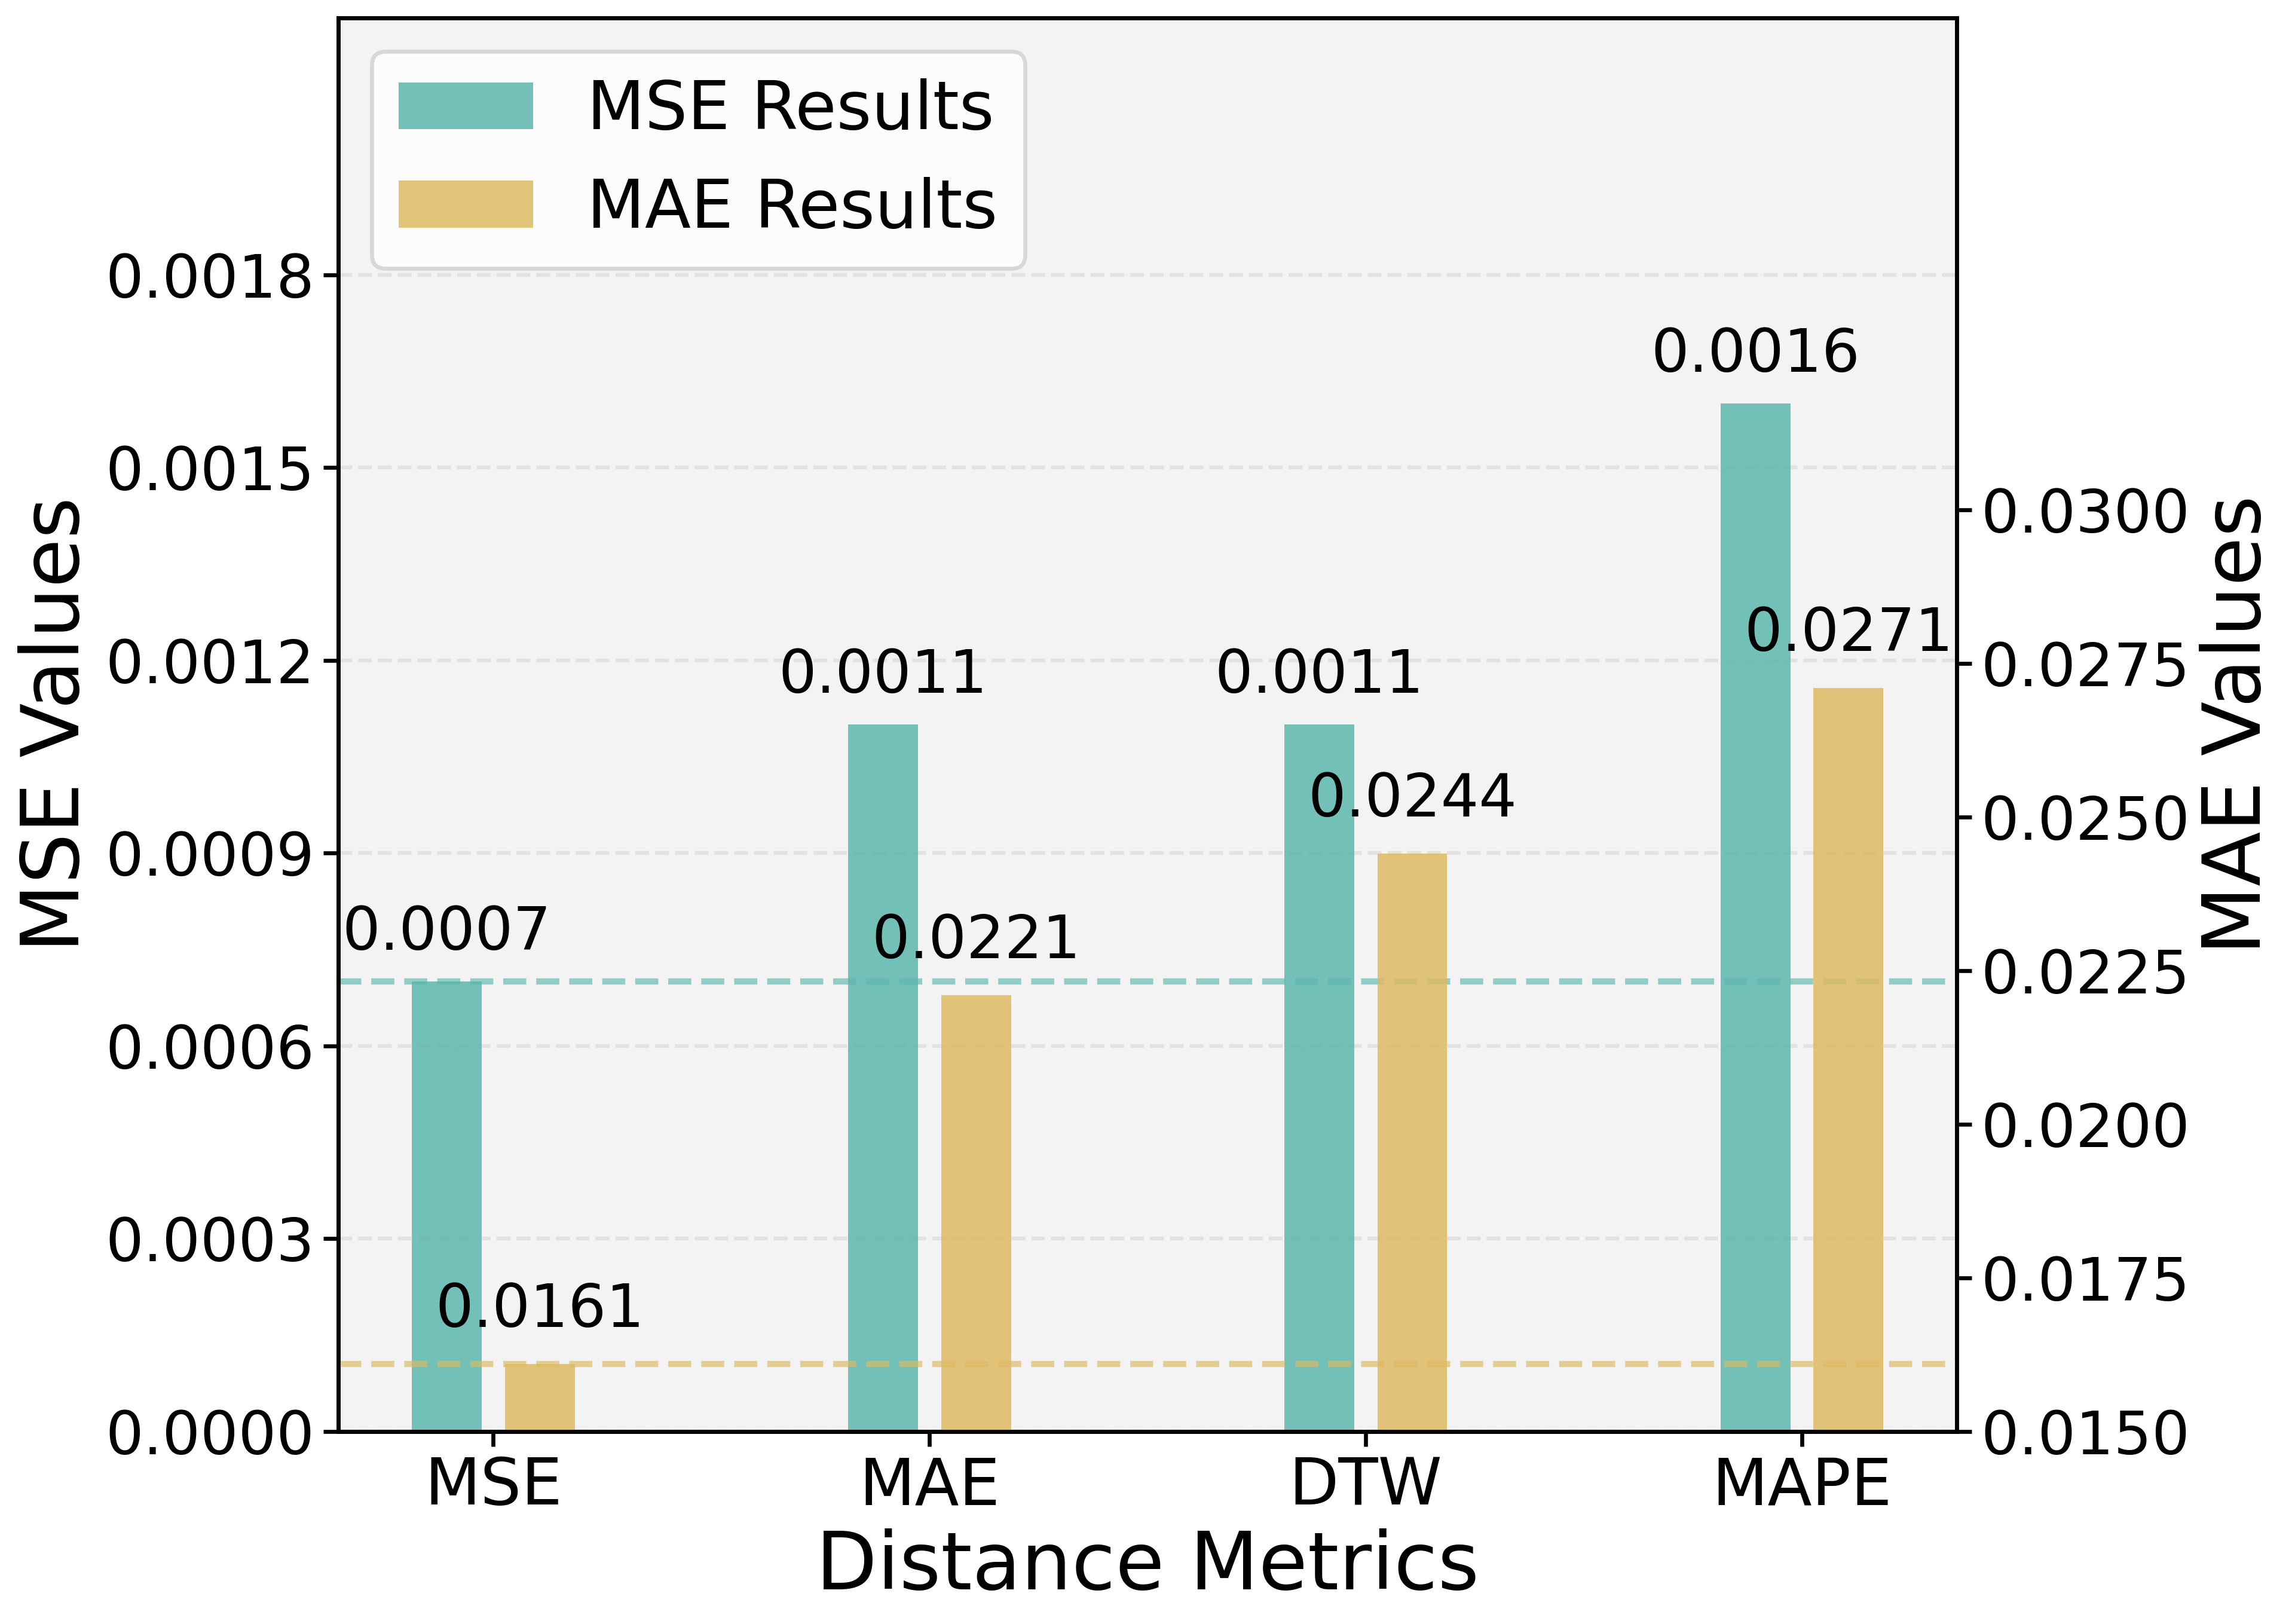
\includegraphics[width=0.32\textwidth]{images/distance/Exchange_results.png}
     \hspace{0.01\textwidth}
    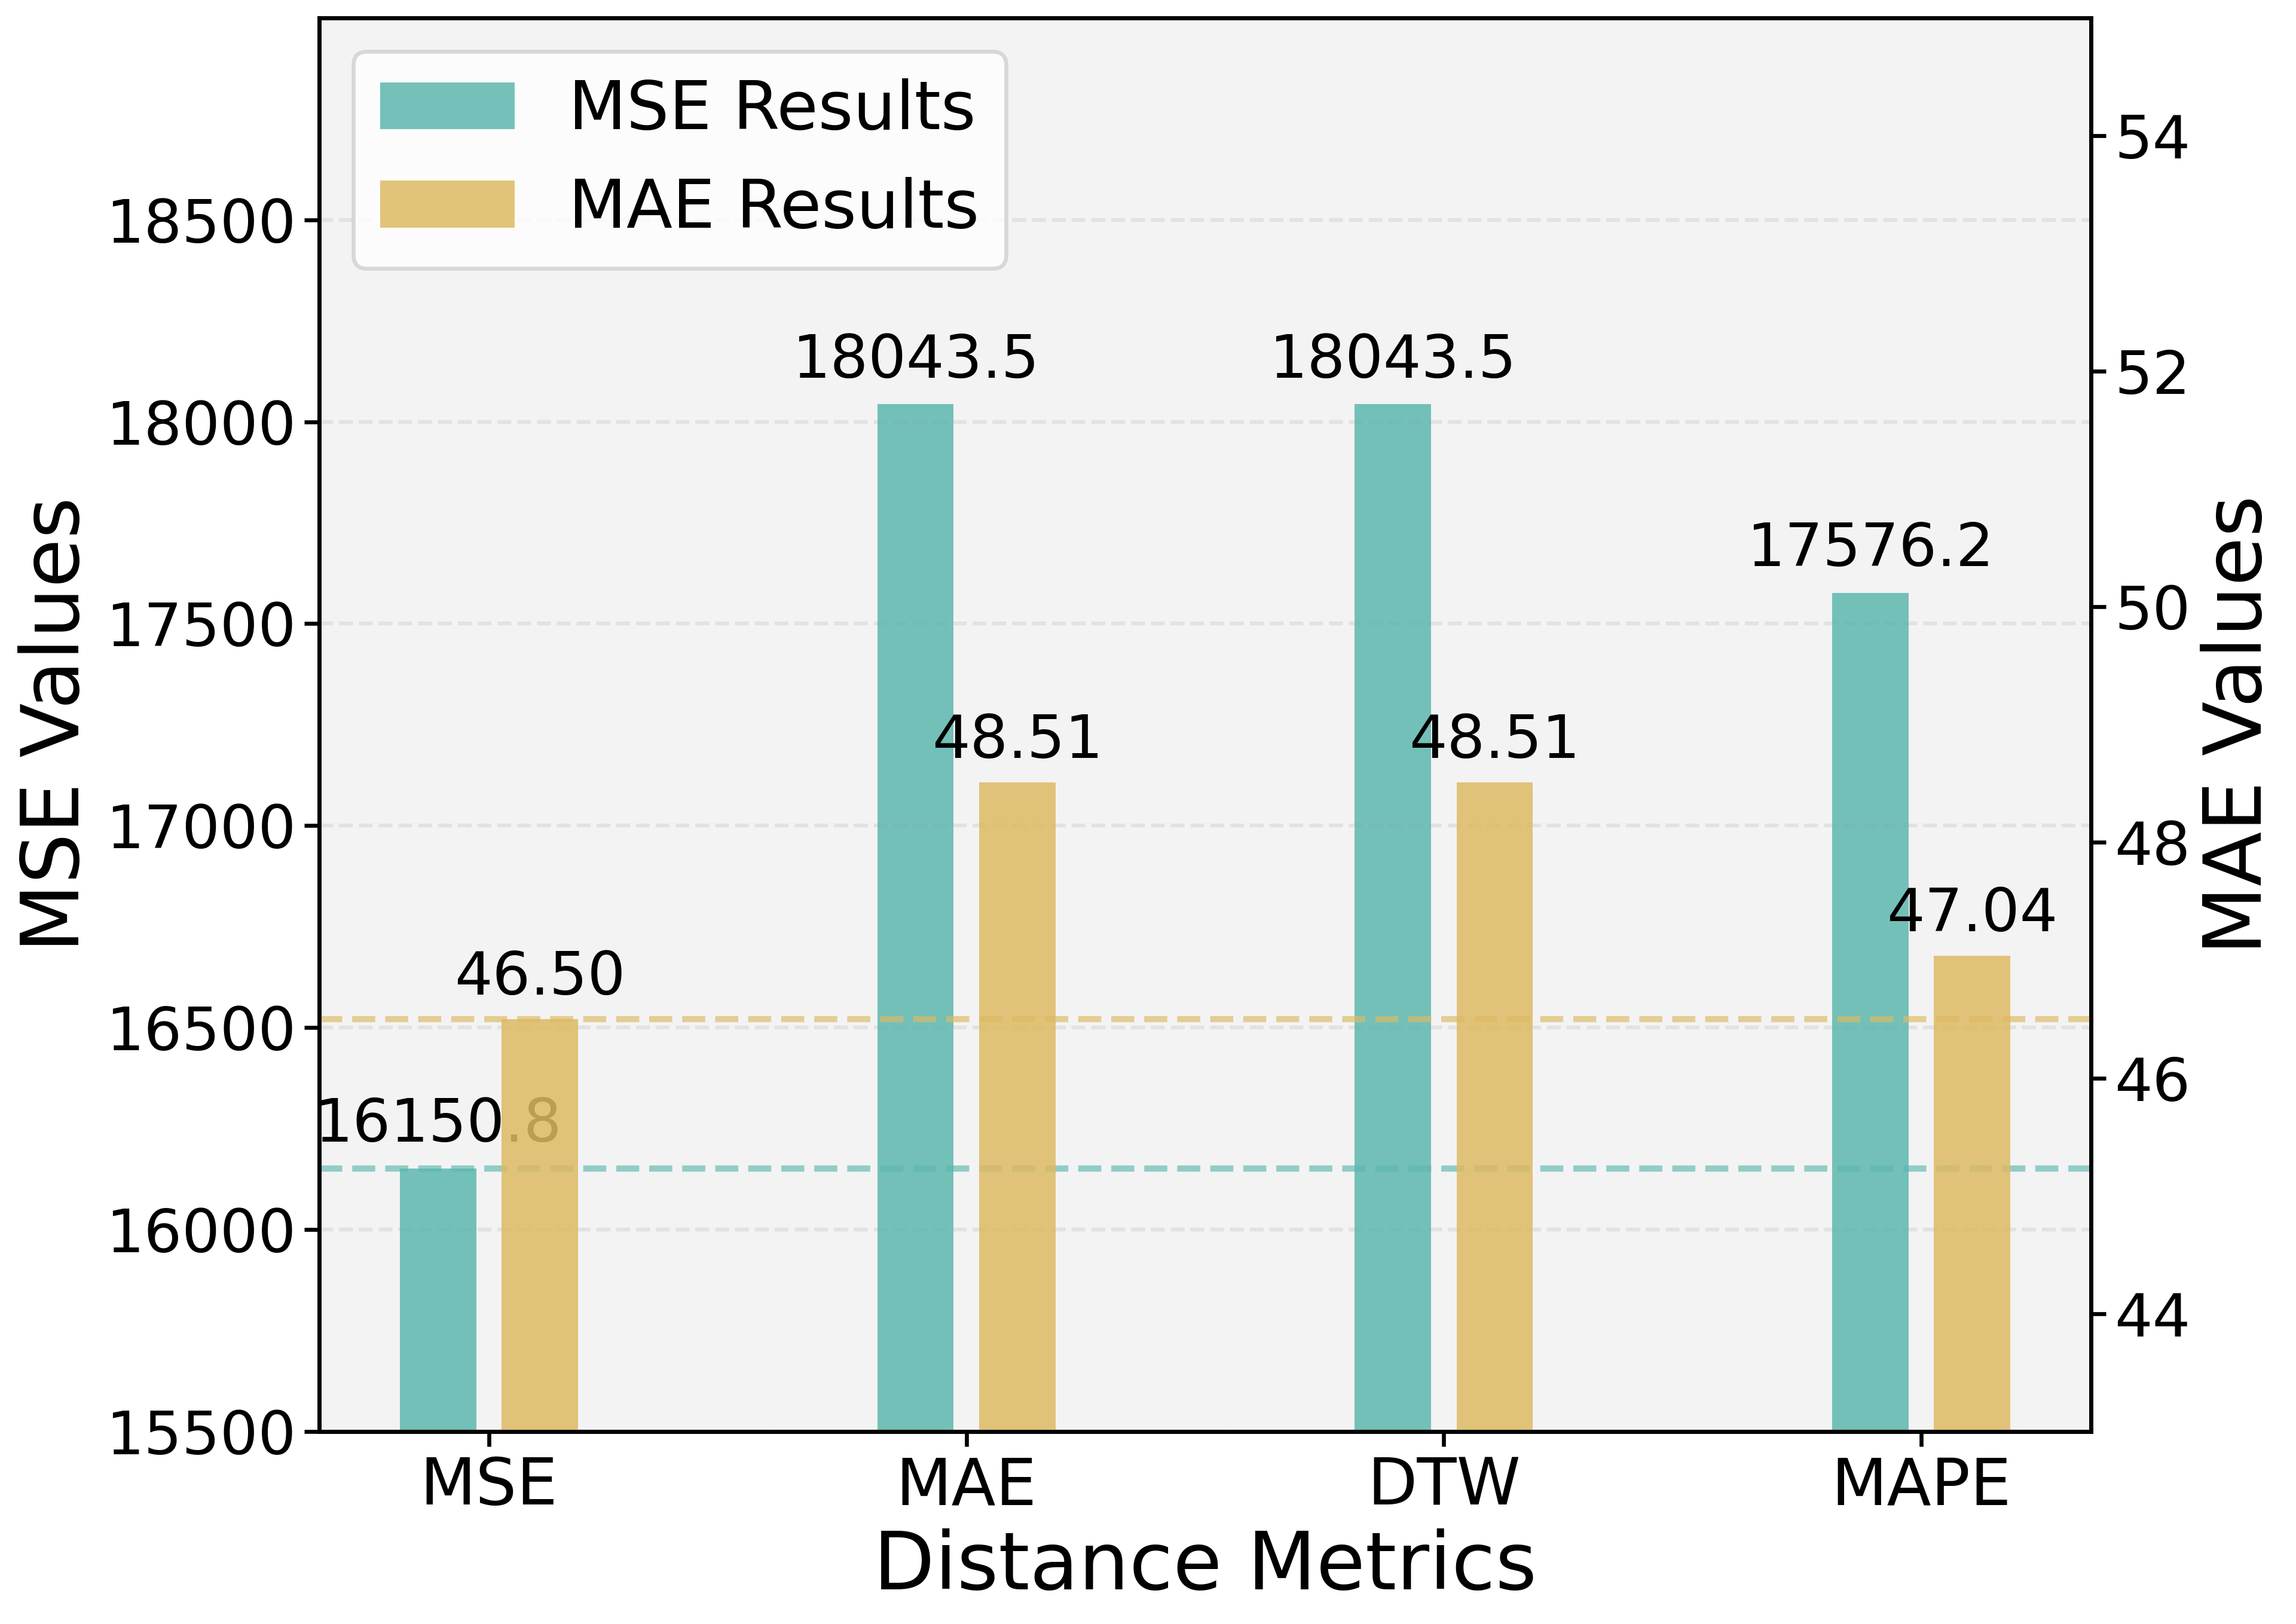
\includegraphics[width=0.32\textwidth]{images/distance/AQShunyi_results.png}
    \hspace{0.01\textwidth}
    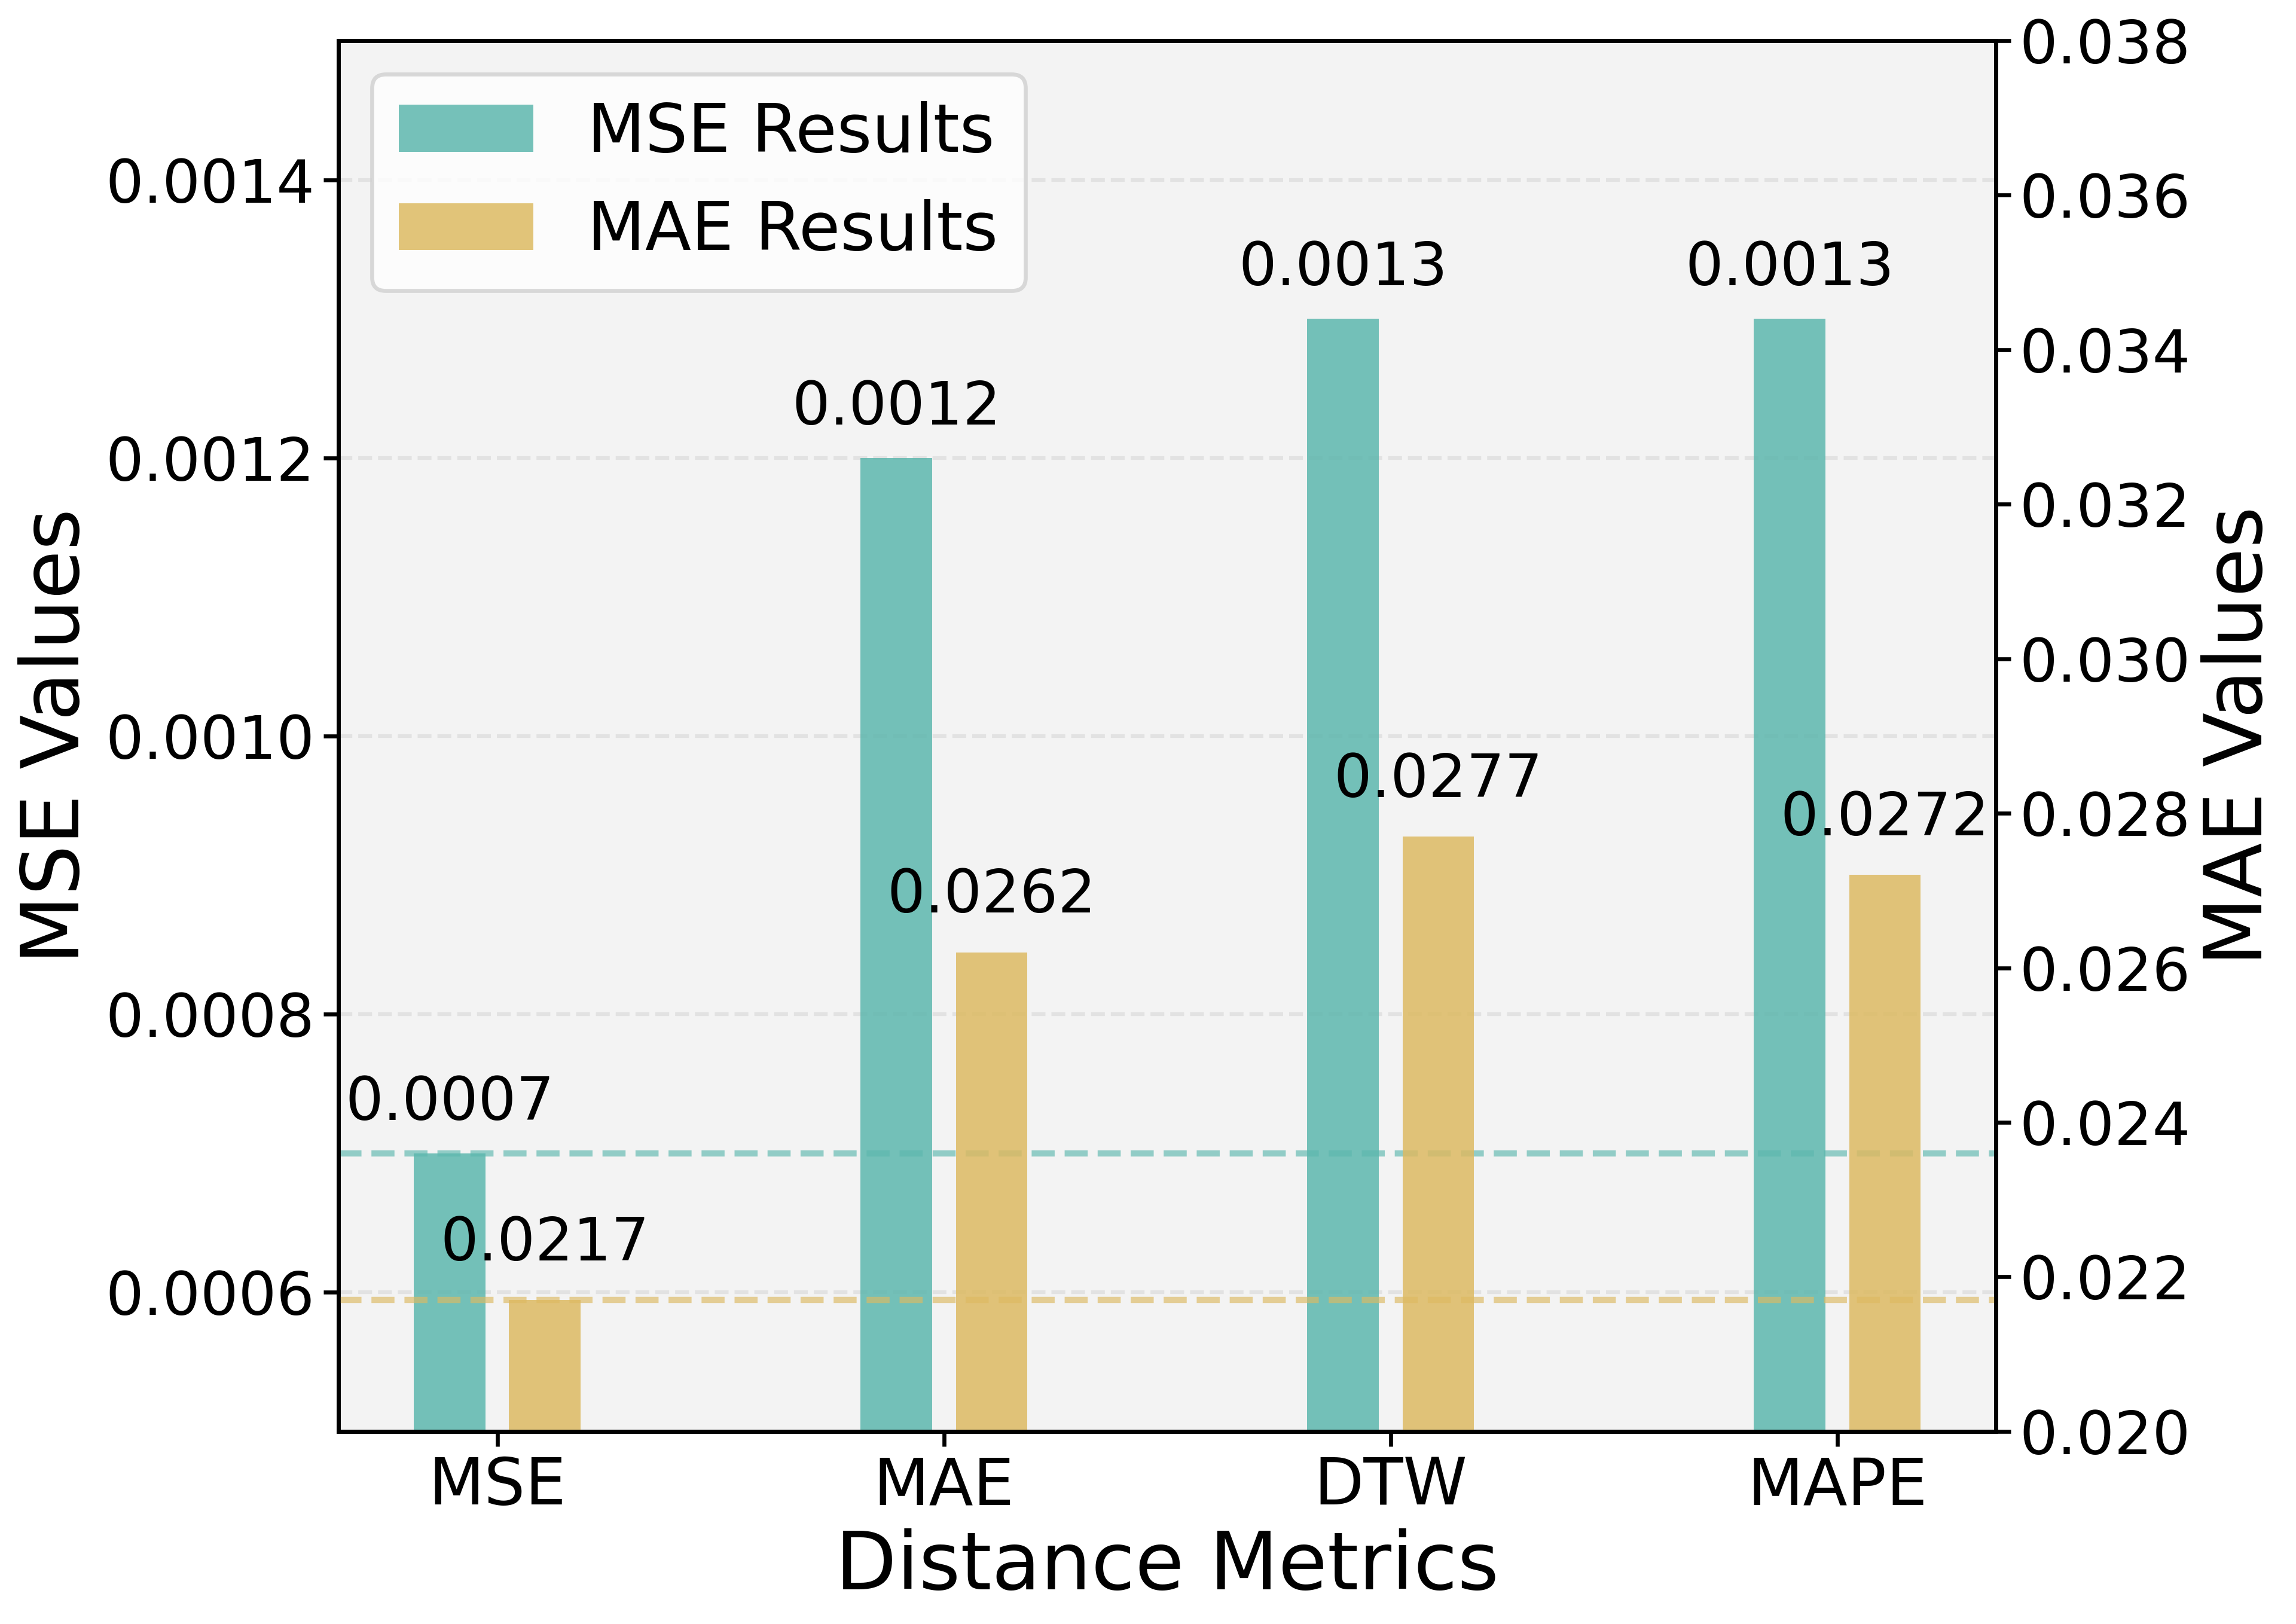
\includegraphics[width=0.32\textwidth]{images/distance/NASDAQ_results.png}
    \vspace{-0.1in}
    \caption{Experimental results based on MSE, MAE, DTW, MAPE Distance Metrics.} 
    \label{fig:distance_metrics}
    \vspace{-0.1in}
\end{figure*}

\vspace{-0.02in}
\subsection{Ablation Study}

% To gain deeper insights into the effectiveness of each component in our proposed \Ours framework, we conduct a comprehensive ablation study across three key aspects: reward design, supervised fine-tuning strategy, and training template components. All ablated variants are evaluated under identical experimental settings to ensure fair comparisons.



\paragraph{Impact of SFT and Reinforcement Learning.}

Next, we evaluate the necessity of CoT-based SFT by comparing two training strategies: (i) direct RL without SFT, and (ii) SFT followed by RL. As illustrated in Figure~\ref{fig:compare}(b), the model trained without SFT suffers from slower convergence and inferior performance, especially in early training stages. In contrast, initializing RL with a well-aligned SFT model significantly accelerates learning and leads to better final performance. This demonstrates that SFT provides a strong foundation for reasoning path generation, which is then further refined through rule-augmented reinforcement learning.

Furthermore, we conducted an ablation study by completely removing RL (see Table \ref{tab:ablation}). The results demonstrate a significant degradation in TSF performance, with absolute performance drops on the ETT and Wind dataset respectively, highlighting RL's crucial role in optimizing SFT-initialized reasoning paths and improving forecasting robustness. This finding indicates that while SFT establishes fundamental reasoning patterns, RL provides indispensable optimization through the following mechanisms: (1) discovering higher-reward reasoning trajectories through exploration, and (2) suppressing plausible-yet-incorrect reasoning paths via reward shaping. Overall, RL proves to be a critical factor in achieving stable and competitive performance.

\begin{table}[t]\centering
    \caption{Reasoning intervention study with No Think, Shuffled Think, and Corrupted Think. $\Delta$ denotes the relative MSE increase over Original Think.}
    \renewcommand{\arraystretch}{1.2}
    \vspace{-0.06in}
    \label{tab:reasoning_intervention}
    \resizebox{0.48\textwidth}{!}{
    \begin{tabular}{lccccccc}
        \toprule
        Dataset 
        & Original 
        & \multicolumn{2}{c}{No Think} 
        & \multicolumn{2}{c}{Shuffled Think} 
        & \multicolumn{2}{c}{Corrupted Think} \\
        \cmidrule(lr){2-2}
        \cmidrule(lr){3-4}
        \cmidrule(lr){5-6}
        \cmidrule(lr){7-8}
        & MSE$\downarrow$ 
        & MSE$\downarrow$ & $\Delta$ (\%) 
        & MSE$\downarrow$ & $\Delta$ (\%) 
        & MSE$\downarrow$ & $\Delta$ (\%) \\
        \midrule
        ETTh1 
        & \textbf{5.8752} 
        & 6.0629 & 3.19 
        & 6.5127 & 10.85 
        & 6.7031 & 14.09 \\
        ETTm2 
        & \textbf{5.6673} 
        & 5.9124 & 4.32 
        & 6.3186 & 11.49 
        & 6.5227 & 15.09 \\
        Wind 
        & \textbf{1353.9381 }
        & 1447.2865 & 6.89 
        & 1590.4173 & 17.47 
        & 1655.2947 & 22.26 \\
        \bottomrule
    \end{tabular}
    }
    \vspace{-0.2in}
\end{table}
% \input{table/4_predicted_window_length}

\paragraph{Impact of Multi-objective Reward Design.}

We analyze the impact of each reward term in RL by training models with partial reward components. As shown in Table~\ref{tab:ablation}, removing any term degrades performance, indicating that all contribute to forecasting accuracy. The largest drops occur when MSE or Seasonal-Trend Decomposition rewards are removed, emphasizing the importance of point-wise precision and temporal structure. While Format and Length rewards have smaller effects on metrics, they ensure output consistency and training stability. Structural Similarity reward further enhances structural fidelity, especially for complex sequences. More experiments are in Appendix \ref{more_reward}.


\paragraph{Impact of Training Template Component.}

Finally, we assess how different elements of our structured prompts affect model behavior. We consider two main components: (i) explicit timestamp encoding, and (ii) contextual information such as seasonal period and task constraints. Table \ref{tab:ablation} shows that incorporating these components consistently improves both forecasting accuracy and generalization capability, especially under zero-shot and out-of-distribution scenarios. Models without timestamp information struggle to capture long-range dependencies, while those lacking contextual guidance often produce logically inconsistent outputs. 

\subsection{RL Optimizer Comparison}


We compare the performance of GRIP using two different sampling strategies — Local Random Sampling, and Cluster-based Random Sampling — against GRPO, a commonly used policy optimization method in reasoning-based reinforcement learning. As illustrated in Figure~\ref{fig:compare}(a), the Cluster-based Random Sampling strategy achieves the highest overall performance, slightly outperforming GRPO. This is attributed to its ability to maintain diversity in trajectory selection by clustering samples based on reward values, which helps preserve potentially informative yet low-reward reasoning paths often ignored by greedy methods. In terms of convergence speed, Cluster-based Sampling also leads, followed by Local Sampling, and finally GRPO, which converges the slowest. Although local Sampling explores a larger search space, it tends to overfit high-reward trajectories early on, leading to relatively poor generalization and suboptimal performance.

\begin{figure*}[htp]

    \centering
    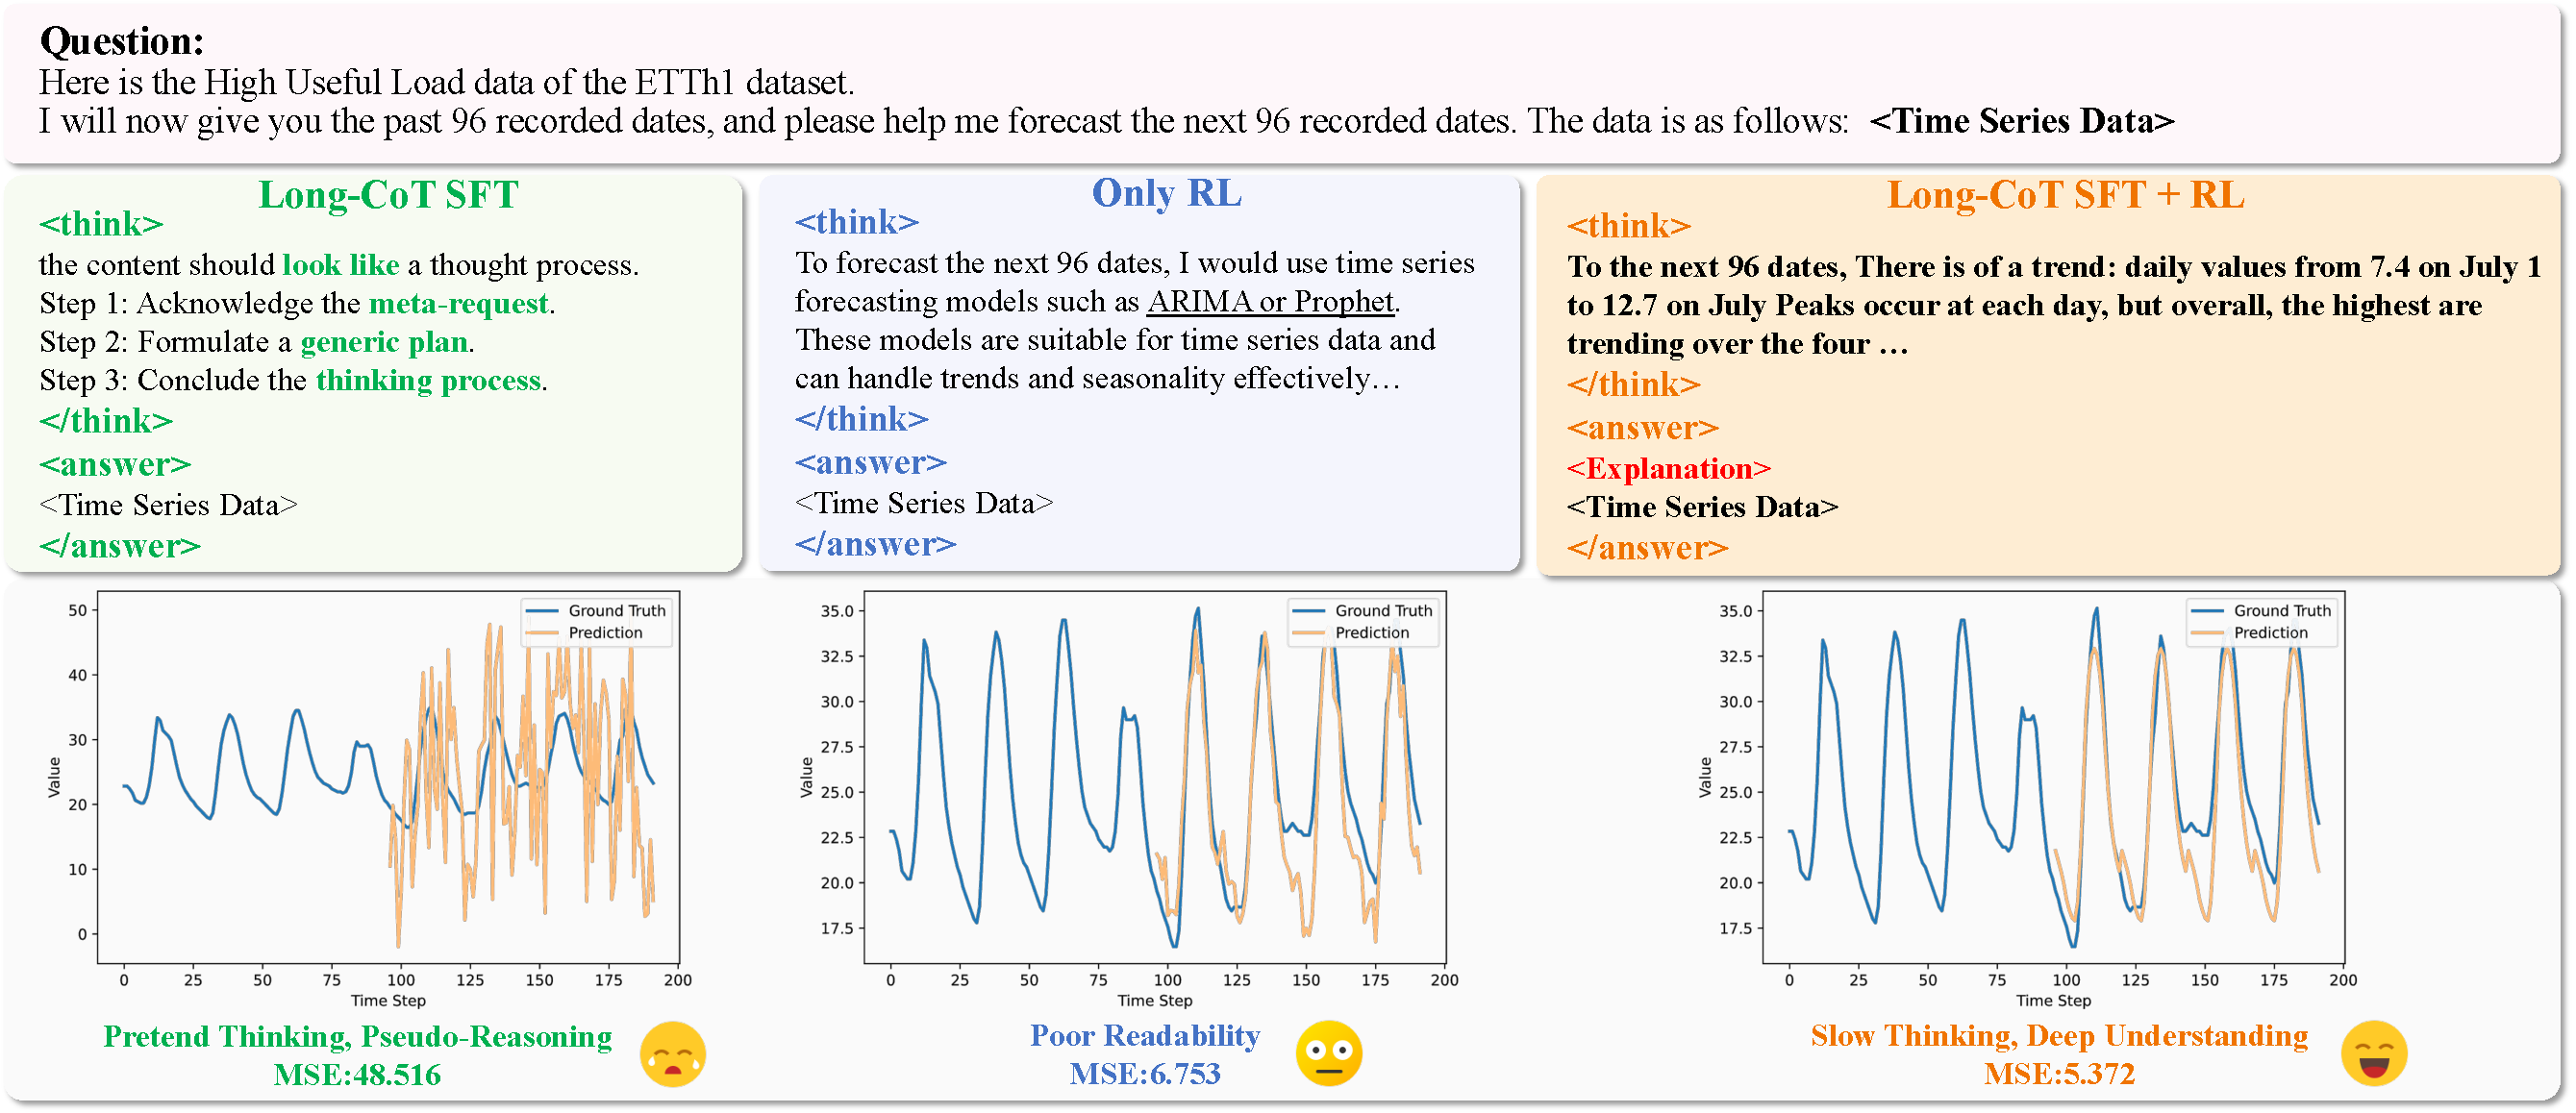
\includegraphics[width=1\textwidth, keepaspectratio]{images/4_reasoning_case_.pdf} 
    \vspace{-0.1in}
    \caption{A reasoning case study of long-CoT SFT, RL, and Hybrid Methods on ETTh1 dataset.}
    \vspace{-0.1in}
    \label{fig:reasoning_case}

\end{figure*}


\vspace{-0.04in}
\subsection{Performance Comparison w.r.t Model Types}

We analyze the training dynamics of \Ours across model types, comparing base and instruct models. Using two Qwen2.5 variants, Qwen2.5-7B-Base and Qwen2.5-7B-Instruct. Figure \ref{fig:compare}(c) shows the base model converges more slowly and starts from a lower performance level. However, it demonstrates stronger learning potential and eventually achieves slightly better results. This suggests that while instruction tuning accelerates early learning in time series reasoning, iterative RL-based optimization enables the base model to reach marginally superior performance.

\vspace{-0.04in}
\subsection{Impact of Accuracy Reward Metrics}
\label{more_reward}
% \paragraph{Distance Metric in Accuracy Reward.}
To examine the choice of accuracy reward in GRIP, we compare four distance metrics, including MSE, MAE, DTW, and MAPE, on the Exchange, AQShunyi, and NASDAQ datasets, as shown in Figure~\ref{fig:distance_metrics}. Overall, MSE yields the best performance across datasets, with MAE ranking second, while DTW and MAPE bring relatively limited gains. This suggests that an effective accuracy reward should provide a stable and discriminative signal that is well aligned with the final forecasting objective. Compared with MAE, MSE more strongly penalizes large deviations and therefore better guides the model to reduce severe multi-step forecasting errors. In contrast, DTW focuses on shape alignment but may weaken point-wise accuracy, and MAPE can be unstable when target values are close to zero. Based on these observations, we adopt MSE as the primary accuracy reward in our framework.


\subsection{Performance Comparison w.r.t Model Sizes} 

To evaluate the scaling behavior of \Ours, we conduct experiments using models with 1.5B, 3B, and 7B parameters on TSF tasks. As shown in Figure~\ref{fig:compare}(d), forecasting performance consistently improves with increasing model size. The 1.5B model achieves reasonable results on simple datasets but struggles with complex temporal patterns. In contrast, the 3B model demonstrates significantly better accuracy and generalization, suggesting that moderate scaling already brings noticeable gains in temporal modeling. The 7B model achieves the best overall performance, particularly in capturing long-term dependencies and handling out-of-distribution scenarios. These results indicate that larger models can substantially enhance temporal reasoning capabilities and that \Ours can effectively benefit from stronger backbone models.

% To evaluate the scaling behavior of \Ours, we conduct experiments using models with 1.5B, 3B, and 7B parameters on TSF tasks. As shown in Figure~\ref{fig:compare}(d), forecasting performance consistently improves with increasing model size. The 1.5B model achieves reasonable results on simple datasets but struggles with complex temporal patterns. In contrast, the 3B model demonstrates significantly better accuracy and generalization, while the 7B model achieves the best overall performance, particularly in capturing long-term dependencies and handling out-of-distribution scenarios. These results indicate that larger models can substantially enhance temporal reasoning capabilities.



% \subsection{Impact of Predicted Window Length}

% Table~\ref{tab:predicted_window} evaluates the robustness of \Ours under extended prediction horizons. As the forecasting window becomes longer, models are more likely to suffer from accumulated errors and trajectory drift. Across all datasets and horizons, \Ours consistently achieves lower MSE than TimeLLM, indicating that the proposed reasoning-oriented optimization better suppresses large forecasting deviations in long-range prediction. This advantage is especially clear on ETTh1, ETTh2, and ETTm1, where \Ours improves both MSE and MAE over different horizons. Although TimeLLM obtains slightly lower MAE on ETTm2 under the 192- and 336-step settings, the differences are marginal, and \Ours still maintains lower MSE. These results suggest that \Ours provides more stable long-horizon forecasting by better controlling accumulated prediction errors and preserving the overall temporal trajectory.


\subsection{Reasoning-Format Intervention Study}
To examine whether explicit reasoning learned during training contributes to forecasting performance, we conduct a reasoning-format intervention study. For the No Think variant, we modify the format reward so that the model is no longer encouraged to generate any explicit reasoning process within \texttt{<think>...</think>}, but instead directly outputs the forecast in \texttt{<answer>...</answer>}. 

In addition, to further test whether the content of reasoning affects the subsequent prediction, we construct two reasoning-perturbation settings at inference time. In Shuffled Think, we first collect the original \texttt{<think>} outputs generated by Time-R1 on the test set, and then replace the reasoning of each sample with a randomly selected \texttt{<think>} from another sample within the same dataset, while keeping the current historical input unchanged. This creates fluent but input-mismatched reasoning. In Corrupted Think, we rewrite the original reasoning of the current sample by reversing key temporal conclusions, such as changing increasing trends to decreasing trends, weakening or removing identified seasonality, and reversing volatility or level-shift descriptions, while preserving the overall format and style. As shown in Table~\ref{tab:reasoning_intervention}, Original Think consistently achieves the lowest MSE across ETTh1, ETTm2, and Wind, while removing, mismatching, or corrupting the reasoning process leads to performance degradation. These results suggest that the explicit reasoning behavior encouraged during training is meaningfully associated with forecasting accuracy, and that the reasoning content is not merely a superficial explanation but can influence the final numerical prediction.

\subsection{Visualization of the Reasoning Process}



As shown in Figure \ref{fig:reasoning_case}, our case study highlights key differences among training paradigms. SFT enables imitation of reasoning patterns but often results in superficial replication, leading to flawed logic and suboptimal performance. Pure RL achieves reasonable accuracy but generates reasoning traces with poor readability. In contrast, the SFT+RL paradigm not only teaches extended reasoning effectively but, through its reinforcement phase, also improves prediction accuracy while helping the model identify which reasoning components most contribute to performance gains.
